% !TeX spellcheck = cs_CZ
% file: prechod_deje.tex
%{\tikzset{external/prefix={tikz/TEO/}}
% \tikzset{external/figure name/.add={ch10_}{}}
%========= Kapitola: Dynamické pochody v lineárních obvodechů ======================================
\chapter[Přechodné děje]{Dynamické pochody v lineárních obvodech}
\minitoc
  \section{Fyzikální podstata přechodných dějů}
    V obvodu, který je v ustáleném stavu, nechť dojde buďto
    \begin{itemize}
      \item ke změně parametru aktivního prvku (např. připojení nebo odpojení zdroje napětí nebo  
            proudu),
      \item ke změně parametru pasivního prvku (např. zvětšení nebo zmenšení odporu, indukčnosti  
            nebo kapacity),
      \item ke změně topologické struktury (např. přerušení větve, spojení větve nakrátko, připojení 
            další větve).
    \end{itemize}
    Kteroukoliv z uvedených změn dostaneme nový obvod jemuž přísluší nový \emph{ustálený stav}; 
    tento stav však nenastane okamžitě. Zmíněná změna přivede obvod do \emph{ne\-us\-tá\-le\-né\-ho 
    stavu}, v němž odezvy napětí a proudů - nazýváme je \textbf{přechodnými jevy} - se postupně 
    přibližují k hodnotám nového ustáleného stavu. Přechodné jevy, ač - přesně vzato - probíhají v 
    nekonečně dlouhé době, jsou v praxi jevy krátkodobými, neboť odezvy se trvale "dostatečně 
    těsně" přiblíží k hodnotám nového stavu již v poměrně krátké době - v běžných případech jsou to 
    mikrosekundy až milisekundy.

    Naskýtá se otázka, proč odezvy obvodu obecně nepřecházejí z původního do nového ustáleného 
    stavu skokem a proč dochází k neustálenému stavu obvodu. Obvod má elektromagnetickou energii 
    $W(t)$, která je součtem energií elektrického pole kondenzátoru $W_e(t)$ a energií magnetického 
    pole cívek $W_m(t)$. Elektromagnetická energie obvodu
    \begin{equation*}
      W(t)=\sum_kW_{e_k}(t)+\sum_kW_{m_k}(t)
    \end{equation*}
    je tedy funkcí napětí na jeho kondenzátorech a proudů v jeho cívkách. Protože tyto veličiny 
    určují energetický stav obvodu, nazýváme je \textbf{stavovými veličinami}.

    \begin{figure}[ht!]
       \centering
       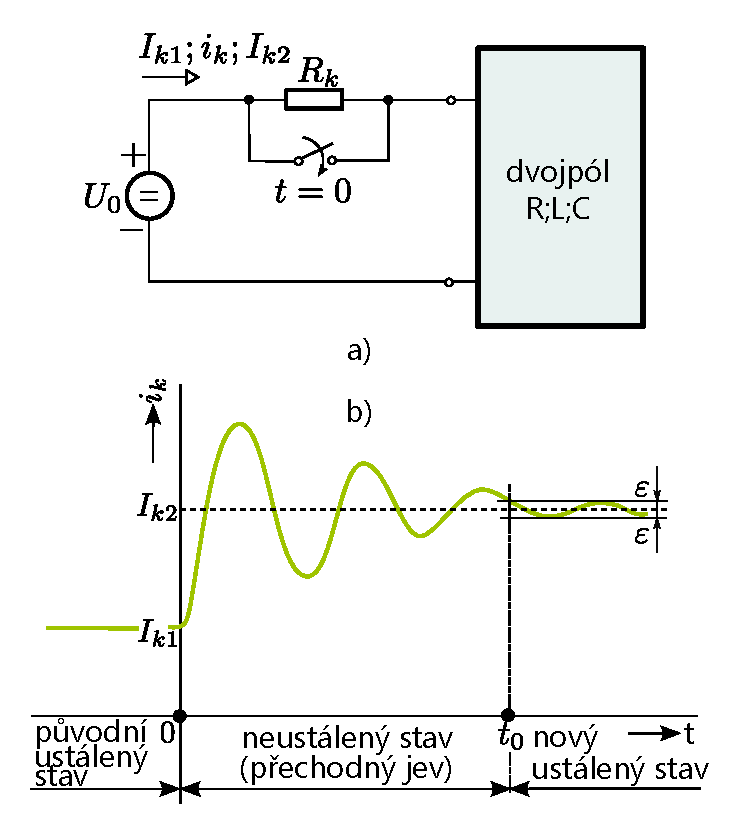
\includegraphics[width=0.8\linewidth]{prechodny_dej.pdf}
       \caption[Přechodný jev]{K objasnění pojmů "neustálený stav" a "přechodný jev"}
       \label{TEO:fig_prechodny_dej}
    \end{figure}

    Elektrické výkony $P$ v reálném elektrickém obvodu mají z fyzikálních důvodů vždy konečnou 
    hodnotu. U obvodů, které jsou dostatečně adekvátními modely respektujícími tuto skutečnost 
    (nazýváme je obvody s konečnými výkony) je to postačující podmínkou pro to, aby jejich energie 
    $W = W(t)$ byla spojitou funkcí času (neboť $P = \frac{dW}{dt}$). Z uvedených vztahů pro 
    energii obvodu $W(t)$ je patrné, že $W = W(t)$ bude spojitou funkcí, jsou-li stavové veličiny 
    \emph{spojitými funkcemi}. To znamená, že hodnota stavových veličin v okamžiku před vznikem 
    přechodného jevu je táž jako v okamžiku po jeho vzniku. Pro přechodný jev v okamžiku $t=0$ 
    platí tedy
    \begin{equation}\label{TEO:eq_spojite_fce}
      \lim_{t\rightarrow0_-}u_c(t)= \lim_{t\rightarrow0_+}u_c(t); \quad  
      \lim_{t\rightarrow0_-}i_L(t)= \lim_{t\rightarrow0_+}i_L(t)
    \end{equation}

     \subsection{Přechodné jevy v jednodušších obvodech; charakteristické pojmy a vlastnosti}
        % --------example: Transformátor -----------------------
        % \label{TEO:exam005}
          % !TeX spellcheck = cs_CZ
\begin{example}\label{TEO:exam005} \textbf{Transformátor}: \newline
  Na primární vinutí vzduchového transformátoru s činitelem $k < 1$ je v čase $t=0$ připojen zdroj 
  napětí $U_1 = konst$. Formulujte postup pro výpočet odezev $i_1(t)$ a $i_2(t)$ pro obecné 
  parametry zapojení a výsledky ověřte simulací pro následující hodnoty: $U_1 = 1V, R_1 = 1\Omega, 
  R_2 = 4\Omega, $ transformátor má převod $1:3$.
  
  {\centering
   \captionsetup{type=figure}
   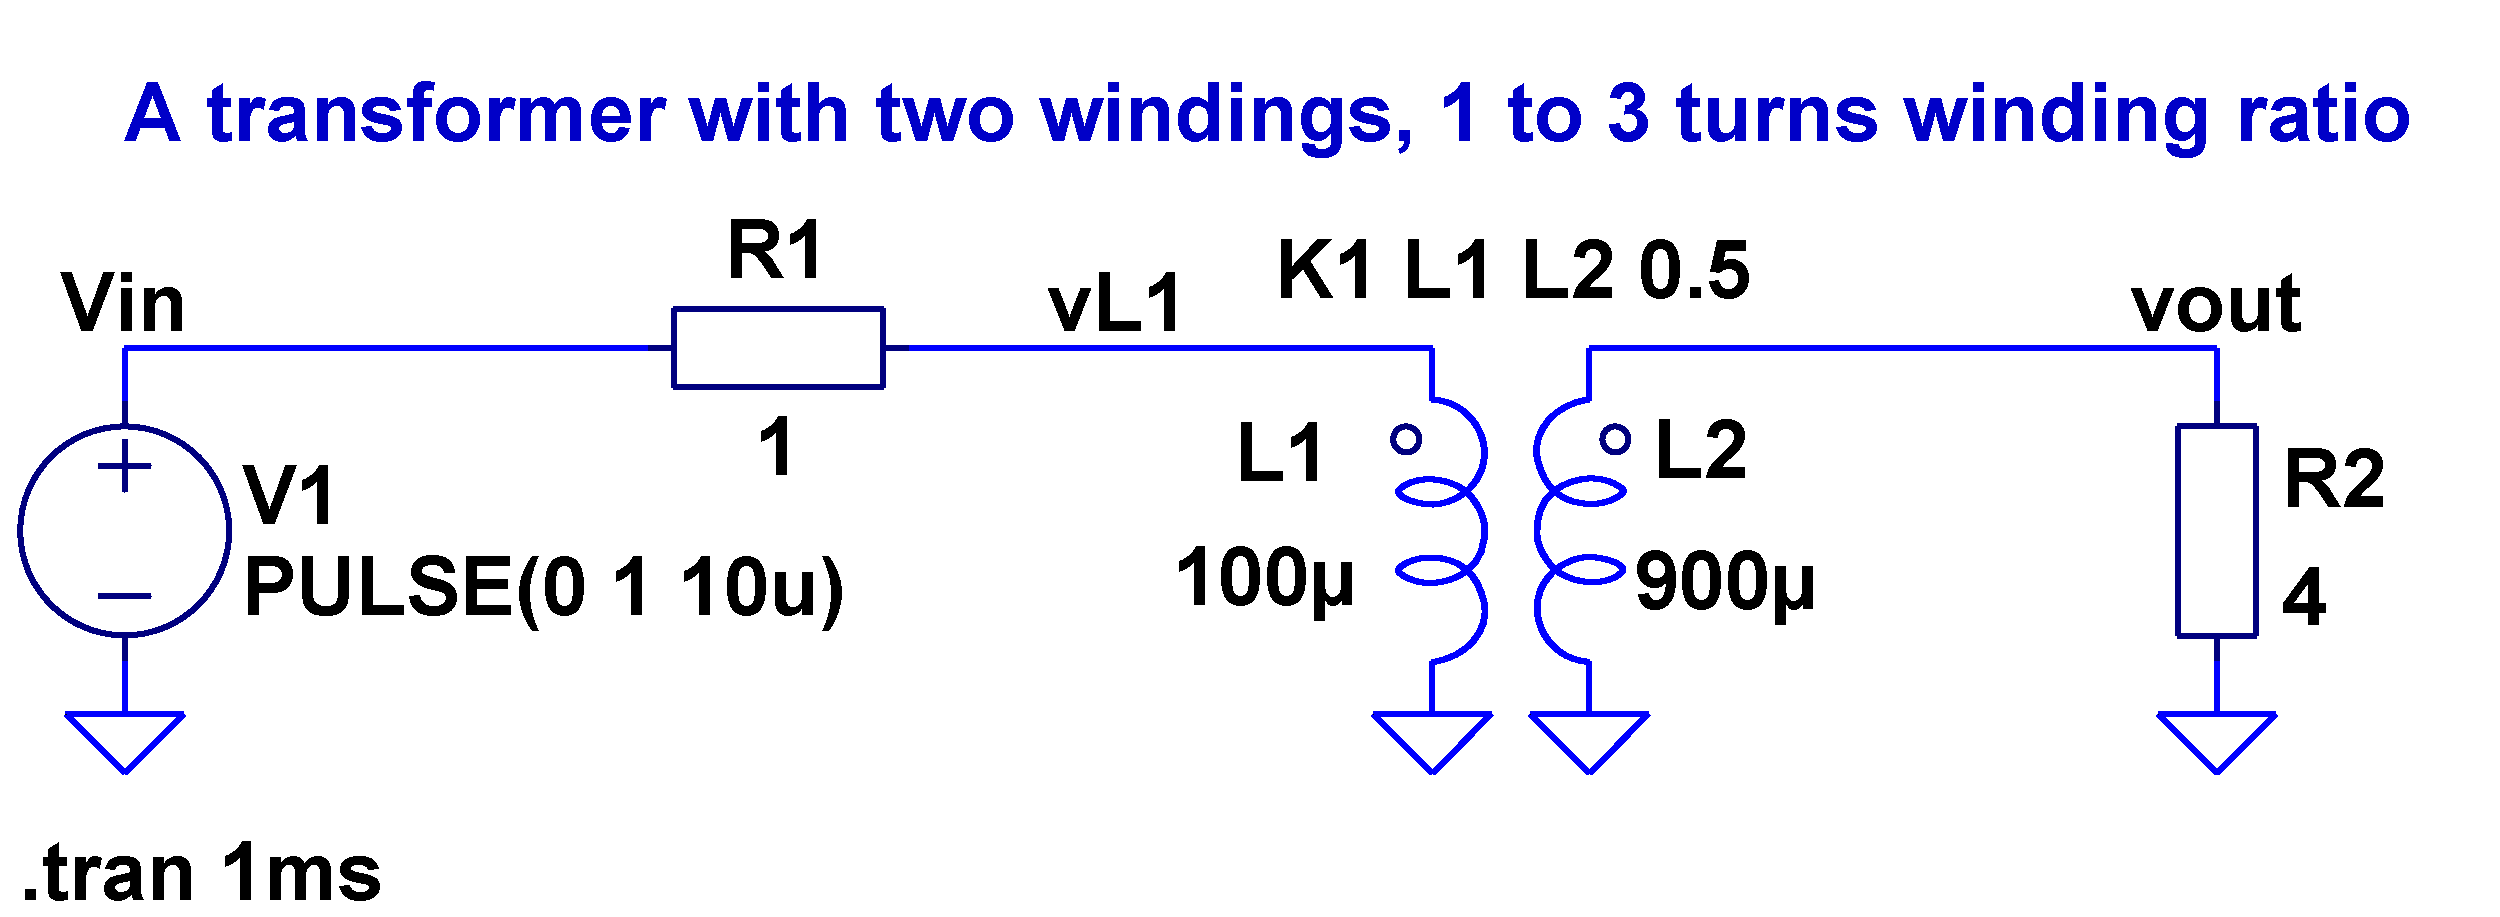
\includegraphics[width=0.9\linewidth]{Ideal_Trf_step_response_LTspice.pdf}
   \captionof{figure}{\texttt{Transformer.asc}: Zapojení vzduchového transformátoru
              pro simulaci v programu LTSpice}
   \label{TEO:fig_trafo_int_uprim}
   \par}
  
  \textbf{Klasické řešení}: Podle II. Kirchhoffova zákona platí soustava rovnic:
  \begin{subequations}\label{TEO:eq_trafo_IIKz}
    \begin{align}
      R_1i_1 + L_1\frac{di_1}{dt} + L_{12}\frac{di_2}{dt} &= U_1 \\
      R_2i_2 + L_2\frac{di_2}{dt} + L_{12}\frac{di_1}{dt} &= 0
    \end{align}
  \end{subequations}
  
  \begin{equation}\label{TEO:eq_char_rce}
  \left(
  \begin{array}{cc}
  R_1 + L_1\lambda & L_{12}\lambda  \\
  L_{12}\lambda    & R_2 + L_2\lambda
  \end{array}
  \right) = 0
  \end{equation}
  \begin{subequations}\label{TEO:eq_char_rce_solve}
    \begin{align}
      (R_1 + L_1\lambda) - L_{12}^2\lambda^2                                      &= 0      \\
      R_1R_2 + (L_1R_2 + L_2R_1)\lambda + L_1L_2\lambda - L_{12}^2\lambda^2       &= 0      \\
      \lambda^2(L_1L_2-L_{12}^2)+(L_1R_2+L_2R_1)\lambda +R_1R_2                   &= L_1L_2 \\
      \lambda^2(\frac{L_1L_2-L_{12}^2}{L_1L_2})+
      (\frac{L_1R_2+L_2R_1}{L_1L_2})\lambda +\frac{R1R2}{L_1L_2}                  &= 0
    \end{align}
  \end{subequations}
  Zavedeme-li $\tau_1 = \frac{L_1}{R_1}, \tau_2 = \frac{L_2}{R_2}$,
  $k=\frac{L_12}{\sqrt{L_1L_2}}, k^2=\frac{L_12^2}{L_1L_2}$, $\sigma = 1-k^2$ dostaneme
  \begin{subequations}\label{TEO:eq_trafo_vysl_rce}
    \begin{align}
      \sigma\lambda^2 + \left(\frac{1}{\tau_1}+\frac{1}{\tau_2}\right)\lambda + 
      \frac{1}{\tau_1}\frac{1}{\tau_2} = 0                                                 \\
      \lambda^2 + \frac{1}{\sigma}\left(\frac{1}{\tau_1}+\frac{1}{\tau_2}\right)\lambda + 
      \frac{1}{\sigma\tau_1\tau_2} = 0
    \end{align}
  \end{subequations}
  Je-li $\lambda_1 = -\beta+\alpha$ a $\lambda_2 = -\beta-\alpha$
  \begin{subequations}
    \label{TEO:eq_trafo_alphabeta}
    \begin{align}
    \alpha &= \frac{1}{2\sigma}
    \left(\frac{1}{\tau_1}+ 
    \frac{1}{\tau_2}\right)            \label{TEO:eq_trafo_alphabeta_a}     \\ 
    \beta  &= \frac{1}{2\sigma}
    \sqrt{\left(\frac{1}{\tau_1}+
      \frac{1}{\tau_2}\right)^2+
      \frac{4\sigma}{\tau_1\tau_2}}      \label{TEO:eq_trafo_alphabeta_b}
    \end{align}
  \end{subequations}
  Jelikož $k<1$; je $0<\sigma<1$; rozborem rovnice \ref{TEO:eq_trafo_alphabeta_b} plyne, že pak
  je $\alpha\neq0$, reálné. Soustava rovnic \ref{TEO:eq_trafo_IIKz} má tedy obecné řešení
  \begin{subequations}\label{TEO:eq_trafo_obecne_res}
    \begin{align}
      i_1(t) &= i_{1o} +i_{1p} = K_1e^{\lambda_1t} + K_2e^{\lambda_2t} +\frac{U_0}{R} \\
      i_2(t) &= i_{2o} +i_{2p} = K_3e^{\lambda_1t} + K_4e^{\lambda_2t}
    \end{align}
  \end{subequations}
  Integrační konstanty $K_1, K_2, K_3$ a $K_4$ určíme z matematických počátečních podmínek:
  $i_1(0)=i_2(0)=0$ (což jsou zároveň fyzikální počáteční podmínky) a $\frac{di_1}{dt}|_{t=0}, 
  \frac{di_2}{dt}|_{t=0}$, které určíme z rovnic \ref{TEO:eq_trafo_IIKz} pro $t=0$:
  \begin{subequations}\label{TEO:eq_trafo_didt_t0}
    \begin{align}
      L_1i_1'+L_{12}i_2' &= U_0 \Longrightarrow i_1' = \left(\frac{U_0-L_{12}i_2'}{L_1}\right)\\
      L_2i_2'+L_{12}i_1' &= 0
    \end{align}
  \end{subequations}
  Dále postupujeme tak, že do druhé rovnice dosadíme vyjádřenou první derivaci primárního
  proudu z první rovnice a získáme vztah pro první derivaci sekundárního proudu v čase $t=0$:
    \begin{subequations}\label{TEO:eq_trafo_dev_i1i2}
    \begin{align}
      \frac{di_1}{dt}|_{t=0} &=   \frac{L_{2}}{L_1L_2-L_{12}^2}U_0                        \\
      \frac{di_2}{dt}|_{t=0} &=  -\frac{L_{12}}{L_1L_2-L_{12}^2}U_0
    \end{align}
  \end{subequations}
  Aplikací těchto počátečních podmínek na obecné řešení \ref{TEO:eq_trafo_obecne_res} plynou
  vztahy
  \begin{subequations}
    \begin{align}
    i_1(0)                            &= K_1 + K_2 +\frac{U_0}{R}                         \\
    \frac{L_{2}}{L_1L_2-L_{12}^2}U_0  &= \lambda_1K_1 + \lambda_2K_2                      \\
    i_2(0)                            &= K_3 + K_4                                        \\
   -\frac{L_{12}}{L_1L_2-L_{12}^2}U_0 &= \lambda_1K_3 + \lambda_2K_4
    \end{align}
  \end{subequations}
  Z první a třetí rovnice vypočítáme $K_1; K_2$, ze druhé a čtvrté rovnice $K_3; K_4$.
  Do\-sa\-ze\-ním do rovnice \ref{TEO:eq_trafo_obecne_res} dostaneme po úpravě odezvy $i_1(t)$
  a $i_2(t)$. Speciálně pro $R_1=R_2=R$;$L_1=L_2=L$ je
  \begin{subequations}\label{TEO:eq_trafo_solved_RL}
    \begin{align}
      i_1(t) &= \frac{U_0}{2R}\left(2-e^{-\frac{t}{\tau_3}}-e^{-\frac{t}{\tau_4}}\right) \\
      i_2(t) &= \frac{U_0}{2R}\left(-e^{-\frac{t}{\tau_3}}+e^{-\frac{t}{\tau_4}}\right)
    \end{align}
  \end{subequations}
  kde je $\tau_3 = \frac{L + L_{12}}{R}; \tau_4 = \frac{L - L_{12}}{R}$
  
  \textbf{Operátorové řešení}: Laplaceovou transformací rovnice \ref{TEO:eq_trafo_IIKz}
  dostáváme
  \begin{subequations}\label{TEO:eq_trafo_laplace}
    \begin{align}
      (R_1 + pL_1)I_1(p)+pL_{12}I_2(p)   &= \frac{U_0}{p} \\
      pL_{12}I_1(p) + (R_2 + pL_2)I_2(p) &= 0
    \end{align}
  \end{subequations}
  Zavedeme $\sigma; \tau_1; \tau_2$, vypočítáme obrazy proudů a jejich zpětnou transformací
  do\-sta\-ne\-me rovnice pro odezvy $i_1(t)$ a $i_2(t)$.
  
  {\centering
   \captionsetup{type=figure}
   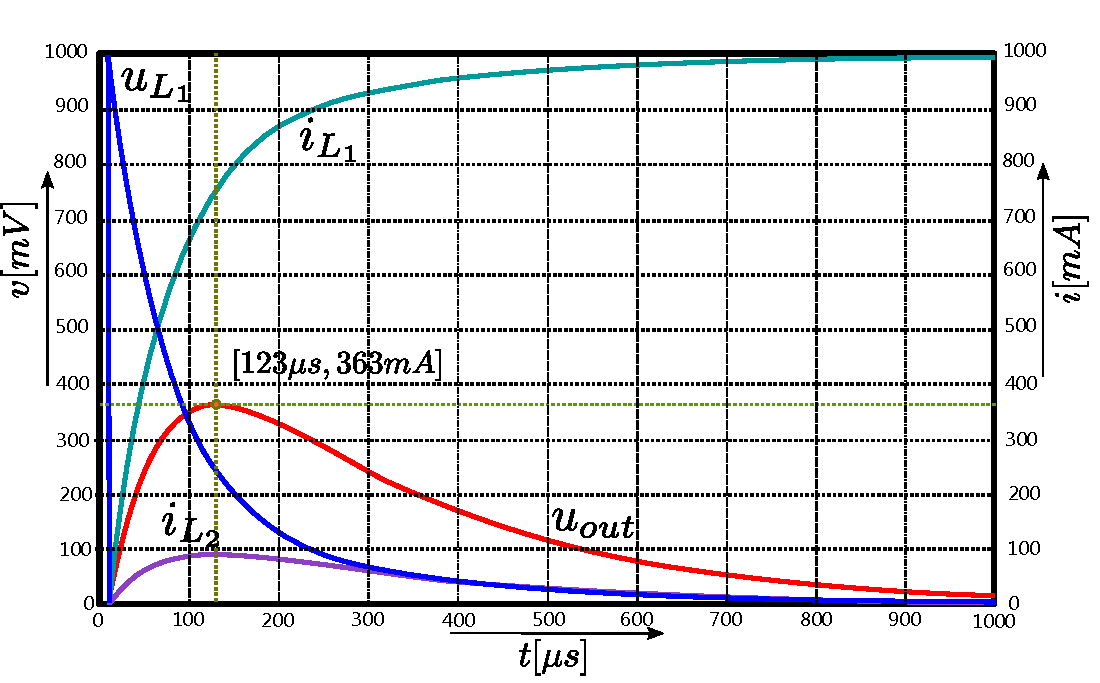
\includegraphics[width=1\linewidth]{Ideal_Trf_step_response_K05.pdf}
   \captionof{figure}{Odezva na jednotkový skok transformátoru s parametry: $k=0.5, L_1 = 100 \mu 
             H, L_2 = 900 \mu H$}
  \label{figure:trafo_int_uprim}
  \par}
\end{example}

  
        %-------------------------------------------------------

        % --------example: Obvod s kondenzátorem ---------------
        % \label{TEO:ex_10_8}
        % % !TeX spellcheck = cs_CZ
\begin{example}\label{TEO:ex_10_8} Najděte odezvu napětí na kondenzátoru $u_c(t)$ obvodu na
  obrázku \ref{TEO:fig_cir_10_8} pro $t>0$. (zdroj \cite[s.~456]{Dorf}) 
  
  {\centering
   \captionsetup{type=figure}
   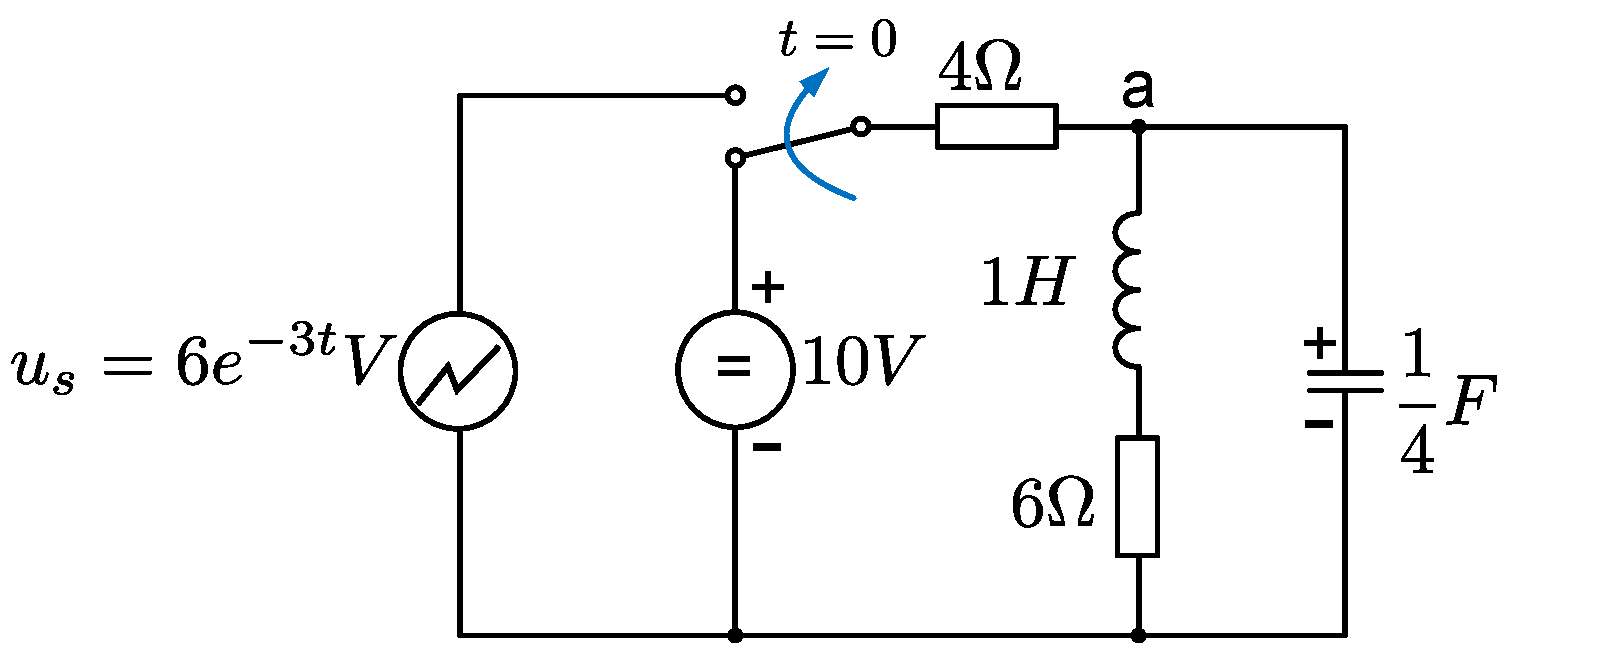
\includegraphics[width=1\linewidth]{response_ex10_8_RLC_cir.pdf}
   \captionof{figure}{Obvod k příkladu \ref{TEO:ex_10_8}}
   \label{TEO:fig_cir_10_8}
   \par}
  
  \textbf{Řešení:} Nejdříve stanovíme počáteční podmínky, které vyplývají z ustáleného stavu
  v době $t = 0^-$. Obvod na obr. \ref{TEO:fig_cir_10_8} můžeme překreslit do podoby na obr.
  \ref{TEO:fig_cir_10_8_steady} 
  
  {\centering
   \captionsetup{type=figure}
   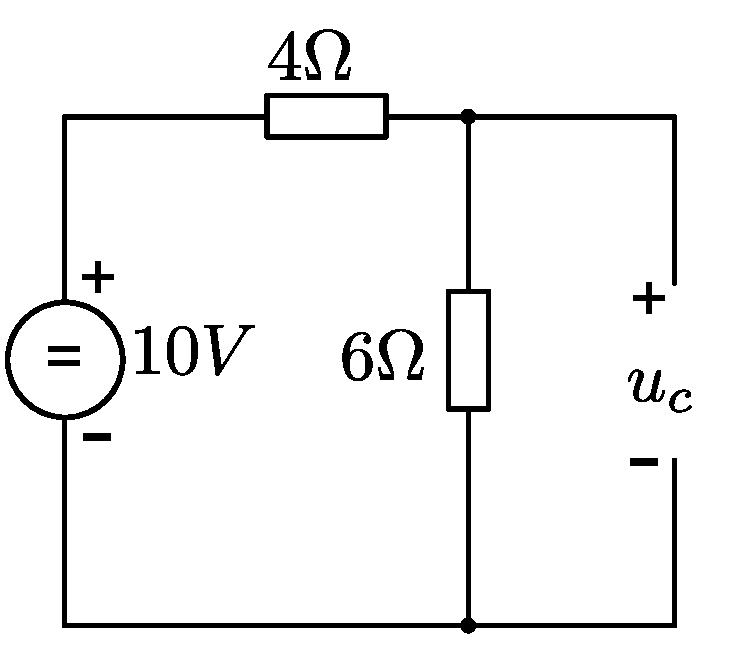
\includegraphics[width=0.4\linewidth]{response_ex10_8_steady.pdf}
   \captionof{figure}{Obvod k příkladu \ref{TEO:ex_10_8}}
   \label{TEO:fig_cir_10_8_steady}
   \par}
  \begin{equation}\label{TEO:eq_10_8_vysledek}
  u_c(t) = \frac{44}{3}e^{-2t}+\frac{1}{3}e^{-5t} - 9e^{-3t} \qquad [V]
  \end{equation}
\end{example}  
        %-------------------------------------------------------
            
  %--------------------- Přechodný jev kmitavého obvodu --------------------------------------------
  \newpage
  \section{Přechodný jev kmitavého obvodu}
    Kmitavým obvodem máme na mysli obvod s jedním stupněm volnosti, složeného z odporu $R$,
    kapacity $C$ a indukčnosti $L$, zapojených v sérii. Je jedním z nejdůležitějších případů
    elektrotechnické praxe. Dosud probírané případy (obvod \emph{RL} a \emph{RC}) jsou vždy určitým
    zjednodušením úplného obvodu s jedním stupněm volnosti, vzniklé tak, že buď indukčnost obvodu,
    nebo kapacita jsou zanedbatelné vzhledem k ostatním prvkům. Rozbor přechodného stavu kmitavého
    obvodu (dále stručně obvodu \emph{RLC}) umožňuje stanovit směrnice pro možnost tohoto
    zjednodušení a jeho důsledky.
    \begin{wrapfigure}{r}{7cm}
      \centering
      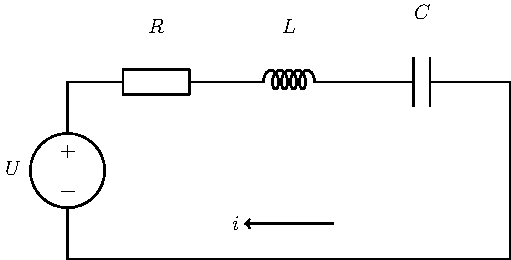
\includegraphics[width=0.45\textwidth]{teo_fig027.pdf}
      \caption[Schéma sériového kmitavého obvodu]{Schéma sériového kmitavého obvodu}
      \label{teo:fig027}
    \end{wrapfigure}
    Zopakujme, že přechodný stav, je vždy dán superpozicí nového ustáleného stavu a vlastní 
    přechodné složky, jejíž průběh závisí jen na vlastnostech obvodu a počátečních podmínkách (a 
    nikoliv na průběhu vstupního signálu), proto nejdříve budeme řešit tzv. \emph{volný stav 
    obvodu}, tj. stav, kdy vnější působení na vstupu je nulové. Za těchto okolností může v obvodu 
    existovat přechodný jev, je-li v obvodu (tj. v akumulačních prvcích) na počátku nahromaděná 
    určitá energie. Vzhledem k tomu, že to může být jednak energie elektrického pole v 
    kondenzátoru, jednak energie magnetického pole v cívce, je počáteční stav úplně určen, známe-li 
    hodnoty napětí na kapacitě a proudu v indukčnosti v počátečním okamžiku; matematicky vyjádřeno, 
    stanovíme počáteční podmínky vždy ve tvaru
    \begin{equation}\label{TEO:eq_RLC_00}
      u_C(0) = U_{C_0} \qquad i(0) = I_0.
    \end{equation}    
    Protože za volného stavu jsou vstupní svorky spojeny \emph{nakrátko}, je rovnice pro proud v
    obvodu
    \begin{align}\label{TEO:eq_RLC_01}
       u_R + u_L + u_C                                    &= 0 \\
       Ri + L\der{i}{t} +\frac{1}{C}\int_0^tidt + U_{C_0} &= 0
    \end{align}     
    Řešení provedeme pomocí Laplaceovy transformace. K přihlédnutím  k počátečním podmínkám
    \ref{TEO:eq_RLC_01} dostaneme rovnici
    \begin{equation}\label{TEO:eq_RLC_02}
      I(p)(R + Lp + \frac{1}{pC}) = I_0L - \frac{U_{C_0}}{p},
    \end{equation}     
    a z ní 
    \begin{equation}\label{TEO:eq_RLC_03}
      I(p) = \frac{pCLI_0 - CU_{C_0}}{p^2LC + pRC + 1}.
    \end{equation}

%} % tikzset
%---------------------------------------------------------------------------------------------------
\printbibliography[title={Seznam literatury}, heading=subbibliography]
\addcontentsline{toc}{section}{Seznam literatury}